\import{./images/solutions}{common}

In der Abbildung \ref{fig:commonSolution} ist der innere Kreis der Architektur dargestellt. Der innere Kreis definiert das Verhalten der Anwendung 
ohne sich auf bestimmte Schnittstellen (z.B. Datenbank oder HTTP) zu binden. 
Die Struktur des inneren Kreises des OCPP Servers ist im Kapitel \ref{Controller-Dispatcher-UseCase-Interactor} beschrieben. 
Der Datenfluss des inneren Kreises ist im Kapitel \ref{kap:Dataflow} beschrieben.
Der innere Kreis wird bei allen Anwednungen ohne jeglichen Änderungen benutzt.

\subsubsection{Controllers}

\begin{enumerate}
    \item \textbf{Super-Controller} besitzt die Aufgabe, den Zugriff auf die anderen \textbf{Contollers} zu ermöglichen. 
    In der Lösung wird das nur von \textbf{UI-Controller} verwendet, somit besteht die Möglichkeit das Programm über \textbf{HTPP-Schnittstelle} zu verwalten. 
    (z.B. Zustände von den \textbf{Controllern} abzufragen).
    \item \textbf{OCPP-Controller} kontrolliert den Websocket-Server, ermöglicht das Abschicken und Aufnehmen von Netzwerk- und OCPP Ereignissen.
    \item \textbf{UI-Controller} kontrolliert den HTTP-Server, ermöglicht das Aufnehmen von HTTP Nachrichten.
    \item \textbf{Logger-Controller} kontrolliert den Zugriff auf das Filesystem, ermöglicht das Logging im Programm.
    \item \textbf{DB-Controller} kontrolliert den Zugriff auf die Datenbank, indem die Verbindung erstellt wird.
    \item \textbf{Chager-Controller} kontrolliert alle Informtationen der bekannten Ladesäulen, 
    ermöglicht folgende Sachen: neue Ladesäule anzulegen, Ladesäuleinformation ändern bzw. löschen, Überprüfen ob gegegbene Ladesäule bekannt ist.
    \item \textbf{User-Controller} kontrolliert alle Informtationen über die bekannten Nutzer der Ladesäulen, ermöglicht folgende Sachen:
    neuen Nutzer anzulegen, Nutzerinformation ändern bzw. löschen, Überprüfen ob gegebene Nutzer bekannt ist.
    \item \textbf{Transaction-Controller} kontrolliert alle Informationen über die Ladevorgänge an den Ladesäulen, 
    ermöglicht folgende Sachen: neue Transaction starten und stoppen.
    \item \textbf{Price-Controller} kontrolliert alle Informationen über den Preis, ermöglicht folgende Sachen:
    Preis für den Nutzer anzulegen und ändern, Standardpreis zu ändern.
\end{enumerate}

\subsubsection{Dispatcher}
Der \textbf{Dispatcher} verteilt die in \textbf{Controllers} aufgetretenen Ereignisse an die UseCases und Interactors, für die das Ereignis zutrifft.

Jedes Ereignis ist eindeutig durch folgende Eigenschaften definiert:
\begin{itemize}
    \item Name des \textbf{Controllers}, in dem das Ereignis aufgetreten ist.
    \item Richtung (vom \textbf{Port} zum \textbf{Controller} oder vom \textbf{Controller} zum \textbf{Port})
    \item Name
    \item Inhalt
\end{itemize}

Es besteht die Möglichkeit Ereignisse im \textbf{Dispatcher} mit Filtern zu abonnieren. 
Zum Beispiel über alle Ereignisse vom bestimmten Controller informieren.

\subsubsection{UseCases}

Jedes Ereignis in jedem \textbf{Controller} wird an Dispatcher weitergegeben, der alle abonnierten \textbf{UseCases} darüber informiert.
Insgesamt gibt es 32 \textbf{UseCases}. 
Davon reagieren 14 auf die Ereignisse vom ``OCPPComm'' Controller und 18 auf die Ereignisse vom ``UI'' Controller. 
Alle anderen \textbf{Controller} definieren keine eigene \textbf{UseCases} auf verschiedene Ereignisse.
Das Defaultverhalten aller Anwendungen ist in den \textbf{UseCases} beschrieben. Es besteht aber die Möglichkeit das Verhalten zur Laufzeit zu ändern, 
dies wird zum Beispiel beim Framework aktiv benutzt.

\newpage
\subsubsection{Interactors}

Der allgemeine Ablauf eines \textbf{Interactors} in der Anwendung:
\begin{figure}[H]
    \centering
    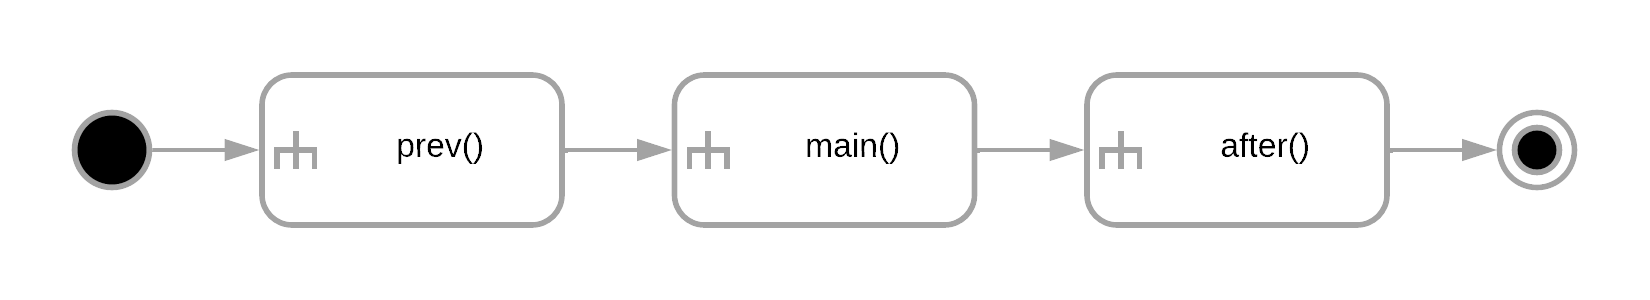
\includegraphics[width=1\textwidth]{./images/InteractorAblauf.png}
    \caption[Ablauf eines Interactors]{Ablauf eines Interactors}
    \label{fig:InteractorFlow}
\end{figure}
Aufbau des \textbf{Interactors}:
\begin{figure}[H]
    \centering
    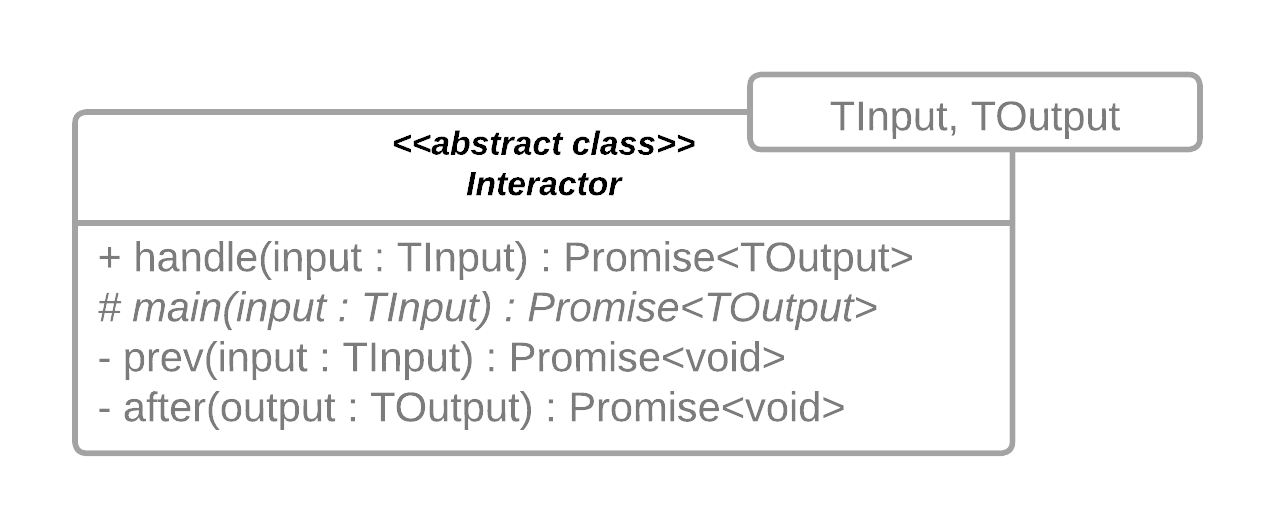
\includegraphics[width=1\textwidth]{./images/InteractorStructur.png}
    \caption[Klassendiagramm eines Interactors]{Klassendiagramm eines Interactors}
    \label{fig:InteractorStructur}
\end{figure}


Fast alle \textbf{Interactoren} hüllen nur Einzelmethoden von \textbf{Controllern} ab.
Es gibt nur ein \textbf{Interactor}, der komplexes Verhalten besitzen.
Das ist:
\begin{itemize}
    \item Abschicken einer OCPP Request Nachricht. Der Rückgabewert ist die Antwort auf die geschickte Nachricht (OCPP Response).
    Siehe Abbildung \ref{fig:dataFlowKomplexInteractor}.
\end{itemize}